\documentclass[a4paper]{article}
\usepackage[a4paper,margin=0mm]{geometry}
\usepackage{fontspec}
\usepackage{unicode-math}
\usepackage{amsmath}
\usepackage{tikz}
\usepackage[table]{xcolor}
\usepackage[absolute]{textpos}
\usepackage{enumitem}
\usepackage{array}
\usepackage{multirow}

\setmainfont{Libertinus Serif}
\setsansfont{Libertinus Sans}
\setmathfont{Libertinus Math}
\newfontfamily\trackedsans{Libertinus Sans}[LetterSpace=8.0]

\definecolor{accent}{HTML}{602785}
\definecolor{badge}{HTML}{B8A0C8}
\definecolor{ink}{HTML}{2A2E30}

\setlength{\TPHorizModule}{1mm}
\setlength{\TPVertModule}{1mm}
\setlength{\parindent}{0pt}
\pagestyle{empty}

\newcommand{\LCOL}{16mm}
\newcommand{\RCOL}{111mm}
\newcommand{\COLW}{83mm}

\newcommand{\topicheader}[2]{%
\begin{textblock*}{194mm}(16mm,10mm)
\begin{tikzpicture}
\node[fill=accent,text=white,font=\sffamily\bfseries\fontsize{13}{13}\selectfont,
      minimum width=9mm,minimum height=9mm,inner sep=0pt] at (4.5mm,-4.5mm) {#1};
\node[font=\sffamily\bfseries\fontsize{15}{16}\selectfont,text=ink,anchor=west] at (12mm,-4.5mm) {#2};
\end{tikzpicture}
\end{textblock*}
\begin{textblock*}{194mm}(16mm,22.5mm)

\begin{tikzpicture}
\fill[accent] (0,0) rectangle (194mm,0.5mm);
\end{tikzpicture}
\end{textblock*}
}

\newcommand{\pagefooter}[1]{%
\begin{textblock*}{194mm}(8mm,286.41mm)
  
\begin{tikzpicture}
    \fill[accent] (0,0) rectangle (194mm,0.6mm);
  \end{tikzpicture}
\end{textblock*}
\begin{textblock*}{63.59mm}(8mm,288.27mm)
  {\sffamily\bfseries\color{accent}\fontsize{13}{16}\selectfont SAT 1200+}
\end{textblock*}
\begin{textblock*}{10mm}(188mm,288.27mm)
  \centering{\sffamily\color{accent}\fontsize{14}{16}\selectfont #1}
\end{textblock*}
}

\newcommand{\colrule}[2]{%
\begin{textblock*}{1mm}(105mm,#1mm)
\begin{tikzpicture}
\draw[black!65,line width=0.5pt] (0,0) -- (0,#2mm);
\end{tikzpicture}
\end{textblock*}
}

\newcommand{\setkicker}[2]{%
{\sffamily\bfseries\fontsize{12}{14}\selectfont #1.}\ {\itshape\fontsize{11}{14}\selectfont\color{black!75} #2}\par\vspace{2mm}%
}

\setlength{\fboxsep}{1.4pt}
\setlength{\fboxrule}{0.5pt}
\newcommand{\pnum}[1]{\fcolorbox{ink}{white}{\sffamily\bfseries\fontsize{8}{8}\selectfont #1}~}

\newcommand{\qrbox}[1]{%
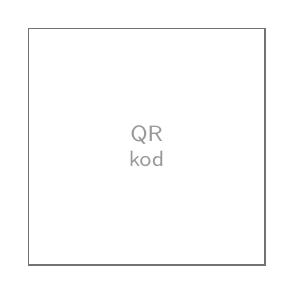
\begin{tikzpicture}
\draw[black!55,line width=0.6pt] (0,0) rectangle (30mm,30mm);
\node[black!40,font=\sffamily\fontsize{8}{9}\selectfont,align=center] at (15mm,15mm) {QR\\kod};
\end{tikzpicture}\\[1.5mm]
{\sffamily\fontsize{9}{11}\selectfont\color{black!70} #1}%
}

\arrayrulecolor{accent}
\setlength{\arrayrulewidth}{0.7pt}
\renewcommand{\arraystretch}{1.35}
\newcommand{\anstitle}[1]{{\sffamily\bfseries\color{accent}\fontsize{11}{13}\selectfont #1}\\[1.3mm]}

\begin{document}

% ================= PAGE 1: Set 1 | Set 2 =================
\topicheader{17}{Ehtimollar nazariyasi asoslari}
\pagefooter{1}
\colrule{32}{238}
\mbox{}%

\begin{textblock*}{\COLW}(\LCOL,32mm)
{\fontsize{11}{14}\selectfont
\setkicker{1-to'plam}{Qulay holatlar / Barcha holatlar.}

\noindent\pnum{1} Xaltada 7 ta qizil, 3 ta ko'k shar bor. $P(\text{qizil})=$\\[16mm]
\noindent\pnum{2} Bankada 5 yashil, 4 sariq, 3 binafsha shar. $P(\text{sariq})=$\\[16mm]
\noindent\pnum{3} 25 nafar o'quvchidan 15 tasi shaxmat o'ynaydi. $P(\text{shaxmat})=$\\[16mm]
\noindent\pnum{4} Aylanada 8 ta teng bo'lak, 1--8 raqamlangan. $P(5\text{ dan katta})=$\\[16mm]
\noindent\pnum{5} Kartalar 1 dan 20 gacha raqamlangan. $P(4\text{ ga karrali})=$\\[16mm]
\noindent\pnum{6} Qutida 6 ta qizil, 9 ta ko'k ruchka. $P(\text{ko'k})=$
}
\end{textblock*}

\begin{textblock*}{\COLW}(\RCOL,32mm)
{\fontsize{10.3}{13}\selectfont
\setkicker{2-to'plam}{Jadvaldan ehtimollik -- avval mos qator/ustunga cheklang.}

\begin{center}
\renewcommand{\arraystretch}{1.25}
\begin{tabular}{|p{14mm}|p{11mm}|p{14mm}|p{9mm}|}
\hline
\rowcolor{badge!45} & \scriptsize Matematikani yoqtiradi & \scriptsize Yoqtirmaydi & \scriptsize Jami\\
\hline
O'g'il & 18 & 12 & 30\\\hline
Qiz & 22 & 8 & 30\\\hline
Jami & 40 & 20 & 60\\\hline
\end{tabular}
\end{center}
\vspace{2mm}

\noindent\pnum{1} $P(\text{matematikani yoqtiradi})=$\\[11mm]
\noindent\pnum{2} $P(\text{qiz})=$\\[11mm]
\noindent\pnum{3} $P(\text{o'g'il VA yoqtiradi})=$\\[11mm]
\noindent\pnum{4} $P(\text{qiz VA yoqtirmaydi})=$\\[11mm]
\noindent\pnum{5} $P(\text{yoqtiradi}\mid\text{o'g'il})=$\\[11mm]
\noindent\pnum{6} $P(\text{qiz}\mid\text{yoqtiradi})=$
}
\end{textblock*}

\clearpage

% ================= PAGE 2: Set 3 | Set 4 =================
\topicheader{17}{Ehtimollar nazariyasi asoslari}
\pagefooter{2}
\colrule{32}{238}
\mbox{}%

\begin{textblock*}{\COLW}(\LCOL,32mm)
{\fontsize{11}{14}\selectfont
\setkicker{3-to'plam}{Birgalikda bo'lmagan hodisalar -- qo'shish qoidasi. Kesishishni tekshiring.}

\noindent\pnum{1} Zar tashlanadi. $P(2\text{ yoki }5)=$\\[16mm]
\noindent\pnum{2} 52 ta kartadan biri tortiladi. $P(\text{Qirol yoki Bibi})=$\\[16mm]
\noindent\pnum{3} Zar tashlanadi. $P(\text{juft yoki }4\text{dan katta})=$\\[16mm]
\noindent\pnum{4} Aylanada 10 ta bo'lak. $P(3\text{ yoki }5\text{ ga karrali})=$\\[16mm]
\noindent\pnum{5} Xaltada 4 qizil, 5 ko'k, 3 yashil. $P(\text{qizil yoki yashil})=$\\[16mm]
\noindent\pnum{6} Zar tashlanadi. $P(3\text{dan kichik yoki toq})=$
}
\end{textblock*}

\begin{textblock*}{\COLW}(\RCOL,32mm)
{\fontsize{11}{14}\selectfont
\setkicker{4-to'plam}{Mustaqil hodisalar -- ko'paytirish qoidasi.}

\noindent\pnum{1} Tanga ikki marta tashlanadi. $P(\text{gerb, gerb})=$\\[16mm]
\noindent\pnum{2} Zar ikki marta tashlanadi. $P(1\text{-si }6\text{ VA }2\text{-si juft})=$\\[16mm]
\noindent\pnum{3} Ikki alohida kolodadan birtadan karta. $P(\text{ikkalasi ham tuz})=$\\[16mm]
\noindent\pnum{4} Aylana 1--4, ikki marta aylantiriladi. $P(1\text{-si toq VA }2\text{-si }4)=$\\[16mm]
\noindent\pnum{5} A xaltada 3 qizil 2 ko'k; B xaltada 4 qizil 6 ko'k. $P(\text{ikkalasi qizil})=$\\[16mm]
\noindent\pnum{6} Og'ir tanga $P(\text{gerb})=0.6$. $P(\text{ikkala tashlashda ham gerb})=$
}
\end{textblock*}

\clearpage

% ================= PAGE 3: Set 5 (classify) | Set 6 (spot the error) =================
\topicheader{17}{Ehtimollar nazariyasi asoslari}
\pagefooter{3}
\colrule{32}{238}
\mbox{}%

\begin{textblock*}{\COLW}(\LCOL,32mm)
{\fontsize{10.3}{13}\selectfont
\setkicker{5-to'plam}{Munosabatni aniqlang: faqat birgalikda bo'lmagan / faqat mustaqil / ikkalasi ham / hech biri emas.}

\noindent\pnum{1} Zar tashlanadi. $A$=juft, $B$=toq.\\[9mm]
\noindent\pnum{2} Ikkita tanga tashlanadi. $A$=1-tangada gerb, $B$=2-tangada raqam.\\[9mm]
\noindent\pnum{3} Kartadan biri tortiladi. $A$=qiyg'ich (heart), $B$=qizil.\\[9mm]
\noindent\pnum{4} Qizil va ko'k zar birga tashlanadi. $A$=qizilda 1, $B$=ko'kda 6.\\[9mm]
\noindent\pnum{5} Kartadan biri tortiladi. $A$=qarg'a (spade), $B$=qiyg'ich (heart).\\[9mm]
\noindent\pnum{6} Zar tashlanadi. $A$=7 tushishi (mumkin emas), $B$=juft son.
}
\end{textblock*}

\begin{textblock*}{\COLW}(\RCOL,32mm)
{\fontsize{10.3}{13}\selectfont
\setkicker{6-to'plam}{Xatoni toping -- mustaqillik va birgalikda bo'lmaslik aralashtirilgan.}

\noindent\pnum{1} $A$=juft, $B$=$4$dan katta. \textit{``Bog'liq emas, shuning uchun $P(A\text{ yoki }B)=\frac36+\frac26=\frac56$.''}\\[1mm]
\hspace*{7mm}Xato va to'g'ri javob: \makebox[50mm]{\dotfill}\\[4mm]

\noindent\pnum{2} Tanga 2 marta. \textit{``Ikkalasi ham gerb g'alati, demak birgalikda bo'lmaydi: $P=0$.''}\\[1mm]
\hspace*{7mm}Xato va to'g'ri javob: \makebox[50mm]{\dotfill}\\[4mm]

\noindent\pnum{3} $A$=2, $B$=5. \textit{``Birgalikda bo'lmaydi, demak mustaqil ham: $P=\frac16\times\frac16$.''}\\[1mm]
\hspace*{7mm}Xato va to'g'ri javob: \makebox[50mm]{\dotfill}\\[4mm]

\noindent\pnum{4} $A$=qizil, $B$=qiyg'ich. \textit{``Ikki xil xossa, demak mustaqil: $P=\frac12\times\frac14$.''}\\[1mm]
\hspace*{7mm}Xato va to'g'ri javob: \makebox[50mm]{\dotfill}\\[4mm]

\noindent\pnum{5} Ikki xaltadan tortish. \textit{``Bog'liq emas, demak birgalikda bo'lmaydi.''}\\[1mm]
\hspace*{7mm}Xato va to'g'ri javob: \makebox[50mm]{\dotfill}
}
\end{textblock*}

\clearpage

% ================= PAGE 4: Set 7 (bonus) =================
\topicheader{17}{Ehtimollar nazariyasi asoslari}
\pagefooter{4}
\colrule{32}{238}
\mbox{}%

\begin{textblock*}{\COLW}(\LCOL,32mm)
{\fontsize{10.5}{13}\selectfont
\setkicker{7-to'plam}{Bonus / qiyin.}

\noindent\pnum{1} 100 kishidan 55 kofe, 40 choy, 20 ikkalasini ham yoqtiradi. $P(\text{kofe yoki choy})=$\\[18mm]
\noindent\pnum{2} $A,B$ mustaqil, $P(A)=0.3$, $P(B)=0.5$. $P(A\text{ yoki }B)=$\\[18mm]
\noindent\pnum{3} Qutida 3 qizil, 7 ko'k. Qaytarmasdan 2 ta tortiladi. $P(\text{ikkalasi qizil})=$\\[18mm]
\noindent\pnum{4} Zar tashlanadi. $A$=$\le3$, $B$=$\ge4$. Birgalikda bo'lmaganmi? Mustaqilmi? $P(A\text{ yoki }B)=$\\[18mm]
\noindent\pnum{5} Ikkita aylana (1--5), mustaqil aylantiriladi. Yig'indi $8$ bo'lish ehtimoli$=$
}
\end{textblock*}

\clearpage

% ================= PAGE 5: Javoblar =================
\topicheader{17}{Ehtimollar nazariyasi asoslari}
\pagefooter{5}
\mbox{}%

\begin{textblock*}{194mm}(16mm,30mm)
{\bfseries\itshape\color{accent}\fontsize{19}{21}\selectfont\centering Javoblar\par}
\end{textblock*}

\begin{textblock*}{194mm}(16mm,42mm)
{\fontsize{9.3}{11.5}\selectfont
\centering
\renewcommand{\arraystretch}{1.3}
\begin{tabular}{|>{\centering\arraybackslash}p{24mm}|>{\centering\arraybackslash}p{9mm}|>{\centering\arraybackslash}p{26mm}|>{\centering\arraybackslash}p{9mm}|>{\centering\arraybackslash}p{26mm}|}
\hline
\rowcolor{badge!55}\textbf{To'plam} & \textbf{\#} & \textbf{Javob} & \textbf{\#} & \textbf{Javob}\\
\hline
\multirow{3}{24mm}{\centering 1-to'plam} & 1 & $\tfrac{7}{10}$ & 2 & $\tfrac13$\\\cline{2-5}
 & 3 & $\tfrac35$ & 4 & $\tfrac38$\\\cline{2-5}
 & 5 & $\tfrac14$ & 6 & $\tfrac35$\\\hline
\multirow{3}{24mm}{\centering 2-to'plam} & 1 & $\tfrac23$ & 2 & $\tfrac12$\\\cline{2-5}
 & 3 & $\tfrac{3}{10}$ & 4 & $\tfrac{2}{15}$\\\cline{2-5}
 & 5 & $\tfrac35$ & 6 & $\tfrac{11}{20}$\\\hline
\multirow{3}{24mm}{\centering 3-to'plam} & 1 & $\tfrac13$ & 2 & $\tfrac{2}{13}$\\\cline{2-5}
 & 3 & $\tfrac23$ & 4 & $\tfrac12$\\\cline{2-5}
 & 5 & $\tfrac{7}{12}$ & 6 & $\tfrac23$\\\hline
\multirow{3}{24mm}{\centering 4-to'plam} & 1 & $\tfrac14$ & 2 & $\tfrac{1}{12}$\\\cline{2-5}
 & 3 & $\tfrac{1}{169}$ & 4 & $\tfrac18$\\\cline{2-5}
 & 5 & $\tfrac{6}{25}$ & 6 & $\tfrac{9}{25}$\\\hline
\multirow{6}{24mm}{\centering 5-to'plam} & \multicolumn{4}{p{70mm}|}{1.\ Faqat birgalikda bo'lmagan ($P(A\cap B)=0\ne P(A)P(B)$).}\\\cline{2-5}
 & \multicolumn{4}{p{70mm}|}{2.\ Faqat mustaqil ($P(A\cap B)=\tfrac14=P(A)P(B)$; HT mumkin).}\\\cline{2-5}
 & \multicolumn{4}{p{70mm}|}{3.\ Hech biri emas (kesishish $\tfrac{13}{52}\ne0$ va $\ne P(A)P(B)$).}\\\cline{2-5}
 & \multicolumn{4}{p{70mm}|}{4.\ Faqat mustaqil (har xil zarlar; $P(A\cap B)=P(A)P(B)$).}\\\cline{2-5}
 & \multicolumn{4}{p{70mm}|}{5.\ Faqat birgalikda bo'lmagan (bir vaqtda ikki xil tur bo'lolmaydi).}\\\cline{2-5}
 & \multicolumn{4}{p{70mm}|}{6.\ Ikkalasi ham ($P(A)=0$ -- chegaraviy holat).}\\\hline
\end{tabular}
}
\end{textblock*}

\clearpage

% ================= PAGE 6: Javoblar (davomi) + QR -- table1 above was already tall =================
\topicheader{17}{Ehtimollar nazariyasi asoslari}
\pagefooter{6}
\mbox{}%

\begin{textblock*}{194mm}(16mm,32mm)
{\fontsize{9.3}{11.5}\selectfont
\centering
\renewcommand{\arraystretch}{1.3}
\begin{tabular}{|>{\centering\arraybackslash}p{24mm}|>{\centering\arraybackslash}p{9mm}|>{\centering\arraybackslash}p{26mm}|>{\centering\arraybackslash}p{9mm}|>{\centering\arraybackslash}p{26mm}|}
\hline
\rowcolor{badge!55}\textbf{To'plam} & \textbf{\#} & \textbf{Javob} & \textbf{\#} & \textbf{Javob}\\
\hline
\multirow{5}{24mm}{\centering 6-to'plam} & \multicolumn{4}{p{70mm}|}{1.\ Kesishish e'tiborga olinmagan (6 soni ham juft, ham $>4$). To'g'ri: $\tfrac36+\tfrac26-\tfrac16=\tfrac23$.}\\\cline{2-5}
 & \multicolumn{4}{p{70mm}|}{2.\ Intuitsiya bilan xato taxmin; HH mustaqil, birgalikda bo'lmagan emas. To'g'ri: $\tfrac12\times\tfrac12=\tfrac14$.}\\\cline{2-5}
 & \multicolumn{4}{p{70mm}|}{3.\ Teskari qoida -- birgalikda bo'lmagan hodisalar mustaqil bo'lolmaydi. To'g'ri: $P=0$, $\tfrac{1}{36}$ emas.}\\\cline{2-5}
 & \multicolumn{4}{p{70mm}|}{4.\ Haqiqiy kesishish e'tiborga olinmagan (har bir qiyg'ich -- qizil). To'g'ri: $P=\tfrac14$, $\tfrac18$ emas.}\\\cline{2-5}
 & \multicolumn{4}{p{70mm}|}{5.\ Mustaqillik ``birga bo'lolmaydi'' degani emas -- alohida xaltalar mustaqillikni bildiradi, birgalikda bo'lmaslikni emas.}\\\hline
\multirow{3}{24mm}{\centering 7-to'plam} & 1 & $\tfrac34$ & 2 & $0.65$\\\cline{2-5}
 & 3 & $\tfrac{1}{15}$ & 5 & $\tfrac{3}{25}$\\\cline{2-5}
 & \multicolumn{4}{p{70mm}|}{4.\ Birgalikda bo'lmagan ($\le3$ va $\ge4$ bir vaqtda bo'lmaydi); mustaqil emas; $P(A\text{ yoki }B)=1$ (butun fazoni qamraydi).}\\\hline
\end{tabular}
}
\end{textblock*}

\begin{textblock*}{194mm}(16mm,220mm)
\centering
{\sffamily\fontsize{9.5}{11.5}\selectfont\color{black!70} Video yechimlar va qo'shimcha testlar uchun quyidagi QR kodlarni skanerlang:}\\[4mm]
\begin{minipage}[t]{32mm}\centering\qrbox{YouTube}\end{minipage}%
\hspace{16mm}%
\begin{minipage}[t]{32mm}\centering\qrbox{Telegram}\end{minipage}
\end{textblock*}

\end{document}
